\documentclass{llncs}
%\usepackage{fancyhdr}
\pagestyle{plain}
%\pagestyle{headings}
\usepackage{standalone}
\usepackage{graphicx} 
\usepackage{comment}
%\usepackage{xcolor}
\usepackage{epigraph}
\usepackage{amsmath}
\usepackage{amsfonts}
\usepackage{amssymb}
\usepackage{cite}
%\usepackage{natbib}
%\usepackage[title]{appendix}
\usepackage{caption}
\usepackage{subcaption}
\usepackage{latexcolors}
\usepackage{import}
\usepackage{tikz}
\usetikzlibrary{positioning}
\usetikzlibrary {arrows.meta}

\newcommand{\red}[1]{\textcolor{red}{#1}}

\begin{document}

%


%\title{Telling the story of best friends}
%
\title{Best friends test: differential importance statistical test reveals hidden specific relations}
%
\titlerunning{Best friends test} 
% abbreviated title (for running head)
% also used for the TOC unless
% \toctitle is used
%
\author{
Alexandra Suvorikova \inst{1} \and Alexei Kroshnin \inst{1} \and Dmirijs Lvovs\inst{6} \and Vasily Ramensky \inst{2,3,4} \and Vera Mukhina \inst{5,6} \and Ludmila Danilova\inst{6} \and Andrey Mironov \inst{4,7} \and Alexander Favorov\inst{6,8}}
%
\authorrunning{A. Suvorikova et al.} % abbreviated author list (for running head)
%
%%%% list of authors for the TOC (use if author list has to be modified)
\tocauthor{Alexandra Suvorikova, Alexey Kroshnin, Dmitrijs Lvovs, Vasily Ramensky, Vera Mukhina, Ludmila Danilova, Andrey Mironov, and Alexander Favorov}
%
\institute{
Weierstrass Institute, Berlin, Germany, 
\email{suvorikova@wias-berlin.de}
\and
MSU Institute for Artificial Intelligence, \\Lomonosov Moscow State University, Moscow, 119992, RF
\and
National Medical Research Center for Therapy and Preventive Medicine of the Ministry of Healthcare of Russian Federation, Moscow, 101990, RF
\and
Department of Bioengineering and Bioinformatics, \\Lomonosov Moscow State University, Moscow, 119992, RF
\and
University of Maryland School of Medicine, Baltimore, MD 21205, USA
\and
Johns Hopkins University School of Medicine, \\ Baltimore, MD 21205, USA, \email{favorov@sensi.org}
\and
The Institute for Information Transmission Problems, Moscow, 127051, RF
\and
Vavilov Institute of General Genetics, RAS, Moscow, 119333, RF
}

\maketitle % typeset the title of the contribution

\renewcommand{\tag}{tag}
\newcommand{\collection}{collection}
\newcommand{\T}{T}
\newcommand{\C}{C}
\newcommand{\tl}{t}
\newcommand{\cl}{c}
\newcommand{\test}[1]{\textbf{\textit{#1}}}

\begin{abstract}
We propose a novel approach to select hidden specific strong connections in a dataset represented by a bipartite graph. \textcolor{red}{...} This model fits many practical problems, such as gene expression regulation by a set of transcription factors, etc. The method is available as an \textsf{R} package at \url{https://github.com/favorov/best.friends}.
\end{abstract}


\keywords{weighted bipartite graph, rank statistics, feature selection, clustering, knowledge transfer, specific gene regulation, pattern marker}

\section{Introduction}

A bipartite graph $G = (V, E)$ is a graph whose set of vertices $V$ can be partitioned into two disjoint subsets $T$ and $C$ such that the union of $T$ and $C$ is equal to $V$ and their intersection is empty, i.e., $
T \cup C = V$,  $T \cap C = \varnothing$.  In a bipartite graph, edges exist only between nodes in $T$ and nodes in $C$; there are no edges connecting vertices within the same subset. \textcolor{blue}{An example is shown at Fig.\ref{fig:nice_name}.} Typically, $T$ and $C$ represent entities of different types, and connections occur only between these distinct types. Consequently, the adjacency matrix $\mathcal{A}_G$ of a bipartite graph $G$ takes the following form,
\begin{equation}
\label{eq:adj_matrix}
\mathcal{A}_G := \begin{pmatrix}
0 & A\\
A^{T} & 0
\end{pmatrix},
\quad
A := \begin{pmatrix}
a_{11} & a_{12} & \dots & a_{1k} \\
 &\cdots & \cdots & \\
a_{n1} & a_{n2} & \dots & a_{nk}
\end{pmatrix},
\quad k := |C|, \quad
n := |T|,
\end{equation}
where $|T|$ and $|C|$ is the number of vertices in $T$ and $C$, respectively. Typically, $a_{ij} = 1$ if there exists an edge between vertices $t_i\in T$ and $c_{j}\in C$, otherwise $a_{ij} = 0$. However, in many practical applications, the weight of an edge may correspond to the distance between nodes, \textcolor{red}{probability that the edge exists}, the strength of the association between the nodes (e.g., correlation), etc. In those cases, the weights $a_{ij}$ are set to real numbers, that is, $a_{ij}\in 
\mathbb{R}$. 

\begin{figure}
 \centering
 \import{}{bipartite}
 \caption{\red{draw a new graph}}
 \label{fig:nice_name}
\end{figure}

The bipartite graph naturally emerges in various real-world settings, including recommender systems \textcolor{red}{[...]}, 
resource allocation problems \textcolor{red}{[...]}, etc.

This model effectively captures intrinsic relationships in complex data structures, such as decomposed omic data \cite{fertig_cogaps_2010, stein-obrien_enter_2018}, \textcolor{red}{phenotype-disease} matrices, and similar datasets. In such problems, the vertices in one part (say, $T$) correspond to features (e.g., genes, phenotypes, etc.), while the vertices in the other part (say, $C$) correspond to the biological processes or conditions (e.g., \textcolor{red}{...}) in which the features participate. The edge weights indicate the association strength: the larger the weight, the stronger the relationship between the corresponding feature and the process.

It is worth noting that the strength of an association can be viewed as the distance between nodes: the stronger the relationship, the smaller the distance. A well-known example is the relationship between correlation and Euclidean distance. Specifically, if association strength is measured as correlation and $r$ is the correlation coefficient between two observations, their Euclidean distance can be calculated as $d = \sqrt{2(1-r)}$. \red{Another well-known example is kernel-based similarity 
calculated from distance [add citation]}. 

The graph-based model described above is well suited for formulating and solving various practical problems. Before introducing the specific problem that this study focuses on, we will briefly recall some related settings.

\paragraph{Assignment problem} In many applications, the aim is to find the pairs of closest nodes $t\in T$ and $c \in C$ \red{[...]}. 
This problem can be naturally stated as the assignment problem \red{[...]}. Let a distance function be $D :T \times C \rightarrow \mathbb{R}_{+} $. The goal is to find the bijection $f: T \rightarrow C$ such that the total distance is minimum, i.e., $\sum_{t\in T}D(t, f(t)) \rightarrow \min_{f}$.

\paragraph{Detection of hubs}
Hubs are nodes with an unusually high degree. By visualizing and analyzing hubs, one can gain insights into how networks represented by graphs are structured \cite{royer2022epilepsy}. In contrast, other studies treat hubs as outliers \cite{kirkley2024identifying}.

\paragraph{Search for specific nodes} In certain applications, the objective is to identify the pairs of nodes satisfying specific properties. Stein et al. \cite{stein-obrien_patternmarkers_2017} examine a set of features $T$ and a set of biological processes 
$C$, in order to pinpoint markers: features that are strongly associated with exactly one process. 

\paragraph{Problem setting}
The current study generalizes the setting introduced in \cite{stein-obrien_patternmarkers_2017}. Our objective is to identify all features that are strongly associated with a few processes. In other words, our goal is to find all nodes in $T$ that are strongly associated to at least one node in $C$, but not with too many of them. In this setting, the association strengths between nodes are edge weights stored in the block $A$ of the adjacency matrix \eqref{eq:adj_matrix}. Throughout the rest of the text, and for the sake of simplicity, we will use the term ``distance'' instead of ``association strength''. 

For generality, we assume the observed processes (vertices in $C$) to be of different natures, making it impossible to directly compare the distance between a fixed node $t\in T$ and arbitrary nodes $c, c' \in C$ \red{provide an example?}.  Moreover, we do not impose any modeling assumptions on the distributions of entries in $A$. This makes it impossible to quantitatively define which nodes in $C$ are ``close'' and which are ``distant'' to $t\in T$. These concepts are therefore relative and depend on the structure of the entire matrix $A$.

To address this challenge, the current study proposes a novel self-tuning approach for identifying vertices $t \in T$ that have only a few close nodes in $C$. In what follows, we present the core ideas behind this procedure, referred to as the \textit{friends.test}.

\subsection{Blueprint of the procedure}
 
Through the rest of the text, we assume that all edge weights $a_{ij} \in A$ (see \eqref{eq:adj_matrix}) are independent random variables. 

\textbf{Step 1: ranking.} First, we apply the ranking to make our approach distribution-free. Specifically, to compare distances between a fixed vertex $t\in T$ and different vertices in $C$, we replace the edge weights $a_{ij} \in A$ with their ranks. Thus, if the ranks of $a_{ij} \in A$ and $a_{ik}\in A$ coincide, we say that $c_k$ and $c_j$ are equidistant from $t_i$.

\textbf{Step 2: model fit.} Next, we filter out the ``equidistant hubs''---vertices in $T$ that are at the same distance to most nodes in $C$. We then fit to the data a parametric model to identify, among the remaining vertices $t\in T$, those that are close to only a few nodes in $C$. The approach is self-tuning. Section~\ref{sec:discussion} discusses a particular choice of the parametric model.

The model fit is performed separately for each vertex $t\in T$ of interest. Since there is typically no an apriori preference for a particular vertex $t$, one can perform model fit for all relevant vertices simultaneously. In this case, the multiplicity correction should be applied. 

\paragraph{Computational aspects.} Denoting the cardinality of $T$ as $n$, and the cardinality of $C$ as $k$ ($|T| = n$, $|C| = k$), one can estimate the computational complexity of \textit{friends.test} as $\mathcal{O}(kn\log(n))$.
\textcolor{red}{The approach suits well for the large data sets.}

\paragraph{R-package}
The software implementing the \text{friends test} is available as an \textsf{R} package \textit{friends.test} at 
\url{https://github.com/favorov/best.friends}. The package vignette shows simple use cases.


\paragraph{The organization of the paper} Section~\ref{sec:method} introduces the \textit{friends.test}. Section~\ref{sec:experiments} presents the experiments. Section~\ref{sec:discussion} discuss...

\section{\textit{Friends}-method}
\label{sec:method}
Denote a set of all observed collections as $C := \{c_1, \dots, c_k\}$, and a set of all observed tags as $T := \{t_1, \dots, t_n\}$.
The attention $A(t_i, c_j)$ is the weight of an edge between $t_i$ in $ T$ and $c_j$ in $C$ (see Fig.\ref{fig:nice_name}).
Let's agree that the greater the $A(t_i, c_j)$, the higher the attention is. Naturally, the absence of attention corresponds to $A(t_i, c_j) = 0$. 

Let $a_{ij} := A(t_i, c_j)$. The corresponding attention matrix is 
\[
\mathcal{A} := \begin{pmatrix}
a_{11} & a_{12} & \dots & a_{1k} \\
 &\cdots & \cdots & \\
a_{n1} & a_{n2} & \dots & a_{nk}
\end{pmatrix}.
\]
Of note, one may think of $\mathcal{A}$ as a non-diagonal block of a weighted adjacency matrix of the bipartite graph.

In what follows we will denote the $i$-th row of the matrix $\mathcal{A}$ as $\text{row}_i(\mathcal{A})$ and its $j$-th column $\text{col}_j(\mathcal{A})$, i.e.,
\[
\text{row}_i(\mathcal{A}) := (a_{i1}, \dots, a_{ik}),
\quad
\text{col}_j(\mathcal{A}) := (a_{1j}, \dots, a_{nj}).
\]
In other words, a row $\text{row}_i(\mathcal{A})$ corresponds to attention that a tag $t_i$ receives from all collections in $C$; a column $\text{col}_j(\mathcal{A})$ corresponds to attention from a collection $c_j$ to all tags in $T$.

In the rest of the text, we assume that all $a_{ij}$ are independent random variables.

Further, under $H_0$ we assume that the attention that each collection $c_j$ from $C$ pays to all tags in $T$ is identically distributed. In other words, values in $\text{col}_j(\mathcal{A})$have the same distribution. We denote it as $P_j$. Typically, all distributions $P_1, \dots, P_k$ are unknown and may vary in nature. 

\subsection*{First step: double ranking}


For each collection $c_j \in C$, we decreasingly rank the elements inside $\text{col}_j(\mathcal{A})$. Thus, for each $a_{ij} $ in $\text{col}_j(\mathcal{A})$, we get the ordinal number $o_{ij}$. \textcolor{red}{We resolve the ties by the mean rank of the tied elements. (ties.method = random)} 

Let $\mathcal{O}$ denote the matrix containing ordinal numbers $o_{ij}$ in place of the corresponding attention values $a_{ij}$, 
\begin{equation*}
\mathcal{O} = \begin{pmatrix}
o_{11} & o_{12} & \dots & o_{1k} \\
 &\cdots & \cdots & \\
o_{n1} & o_{n2} & \dots & o_{nk}
\end{pmatrix}, 
\quad
o_{ij} :=\text{rank}\left(a_{ij}~ \text{inside}~\text{col}_j(\mathcal{A})\right).
\end{equation*}
As before, we denote the $i$-th row of $\mathcal{O}$ as $\text{row}_i(\mathcal{O}) := (o_{i1}, \dots, o_{ik})$.

To quantitatively express the friendliness of all collections to the fixed tag $t_i$, we decreasingly order the ranks stored in $\text{row}_i(\mathcal{O})$. Denote the corresponding rearrangement as $r_{i1}, \dots, r_{ik}$. By construction, $r_{i1} \le r_{i2} \le \dots \le r_{ik}$. Let the corresponding matrix be
\begin{equation}
\label{def:R}
\mathcal{R} := \begin{pmatrix}
r_{11} & r_{12} & \dots & r_{1k} \\
 &\cdots & \cdots & \\
r_{n1} & r_{n2} & \dots & r_{nk}
\end{pmatrix}.
\end{equation}
\paragraph{Idea behind the statistical test} To find the best friends of the tag $t_i$ we are going to split the items inside $\text{row}_{i}(\mathcal{R}) = (r_{i1}, \dots, r_{ik})$ into two non-intersecting groups. One group will match best friends and the other group will match all other collections. 

%NB! Сказать в дискуссии, что метод работает даже если модельное предположение ломается?
\subsection*{Second step: statistical test}
Keeping in mind that now we deal with a single tag $t_i$, let's, for simplicity, omit index $i$. \textcolor{red}{Then,} 
\[
\text{row}_{i}(\mathcal{R}) = (r_{1}, \dots, r_{k}), 
\quad
r_{1} \le \cdots \le r_{k}.
\]

Before proceeding, we must verify that the tag is not indifferent to all collections, e.g. to reject $H_0$. To do this, one can either use a test to assess the homogeneity of the sample $r_{1}, \cdots, r_{k}$ or, alternatively, apply an information criterion, which will be introduced later in the text (see paragraph \textit{Information Criterion})

Assuming a tag has at least one true friend, we aim to split all collections into two groups. A group containing best friends collections, i.e. the collections corresponding to $r_1, \dots, r_{s^*}$ and all the other.

Before introducing a statistical model, we recall two important facts. First, $r_{1}, \cdots, r_{k}$ are independent random variables. Second, each $r_l$ ($1\le l \le k$) takes value ranging from $1$ to $n$. This is because, by construction, each $r_l$ is an ordinal number.

Under $H_1$, we assume that each $r_l$ ($1\le l \le k$) comes from a mixture of two uniform distributions on the discrete grid $1, \dots, n$.
Specifically, the mixture consists of a uniform distribution supported on $1, \dots, m^*$, and a uniform distribution supported on $m^* + 1, \dots, n$, where $m^*$ is an unknown parameter. The probability of each $r \in \{1, \dots, m^*\}$ is $\frac{p^{*}}{m^*}$ and $r \in \{ m^*+1, \dots, n\}$ is $\frac{1 - p^{*}}{n - m^*}$,
see Fig.\ref{fig:model}.
\begin{figure}
 \centering
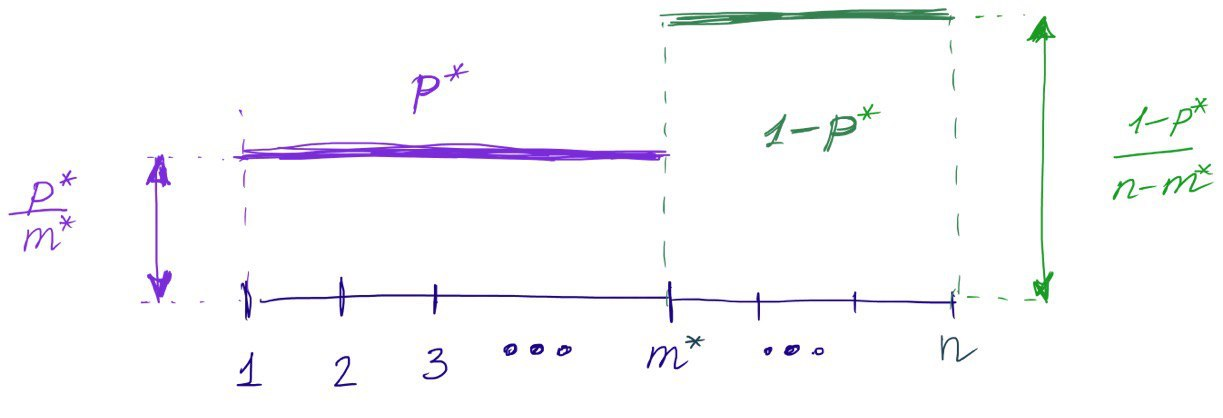
\includegraphics[width=0.8\textwidth]{model.jpeg}
 \caption{....}
 \label{fig:model}
\end{figure}

Note, that $p^*$ and $m^*$ are not known.
We use the maximum likelihood estimation to estimate them based on the observed data $r_1, \dots, r_k$. The likelihood of the mixture is
\[
L(p, m; r_1, \dots, r_k) := s\ln\left(\frac{p}{m}\right) + (k-s)\ln\left(\frac{1-p}{n - m}\right),
\quad
s: r_{s} \le m, ~r_{s+1} > m.
\]
The goal is to find $\hat{p}$ and $\hat{m}$ maximizing $L(p, m; r_1, \dots, r_k)$. Optimizing by $p$ ensures that $\hat{p} = \frac{s}{k}$. All aforementioned ensures that one can use brute-force search over $m$ to find the optimal parameters.

\paragraph{Information criterion}
One can avoid using the homogeneity test by applying the following information criterion.
The approach relies on some preliminary knowledge of the data. Specifically, one has to assume how likely it is that the tag $t$ has friends. We denote the corresponding probability as $q \in (0, 1)$ and set
\[
L_1 := L(\hat{p}, \hat{m}) + \ln(q),
\quad
L_2 := L(0, 0) + \ln(1-q).
\]
The best fit corresponds to $\max\{L_1, L_2\}$.



% \subsection{Symmetric attention matrix $\mathcal{A}$}
% % \textcolor{blue}{\textit{The matrix shows relation tags vs collection and it is not quadratic. How can the non-quadratic matrix be symmetric?}}
% It may happen that the number of tags $n$ coincides with the number of collections $k$, $n = k$. The particular case of the symmetric (by construction) attention matrix $\mathcal{A}$ requires a more detailed investigation.

% The $p$-value calculation relies on the assumption of the independence of attention values in different collections. If the attention matrix $\mathcal{A}$ is symmetric by the nature of the underlying bipartite graph, this assumption \textcolor{red}{does not hold}. Thus, the theoretical inference presented in Section~\ref{sec:theory} is not valid anymore.

% Still, the numerical procedure works. We show this in more detail in Supplement~\ref{seq:symmetric_a}. Of note, sometimes we know that all the diagonal elements are $0$ by construction. In this case, both tests use 
% \[
% p(w) = (1-w)^{k-1}, ~~\text{cf. equation \eqref{eq:pw}.}
% \]


\subsection{Multiple testing}
\label{sec:multimurkers}

All the tests we formulated here are not corrected for the multiplicity of hypotheses. Namely, they work directly if we \textit{a-priori} know what tag $t_i$ and what size $l$ of friends set we run the test for. 

In practice, the tests are run for each tag or even for each tag and the friend set population. Two important observations follow.

\paragraph*{Multiplicity correction} 
To run the \test{best friend test} on all the $n$ tags, we 
calculate $n$ $p$-values. To run the \test{friends test}, we calculate $n \cdot k$ $p$-values. However, all the tests rely on the ranking of the elements inside the same attention matrix $\mathcal{A}$. Thus, the assumption of test independence does not hold. In this case, the standard Bonferroni correction on the set of corresponding $p$-values is possibly too strong (\cite{cabin2000bonferroni}). However, some correction is still necessary. We leave it to the scope of the particular application.

\paragraph*{Multimarkers} Note that after the multiple hypothesis correction, a collection may be the best friend (or an element of the true friends set) for more than one tag. The set of tags is thus a multimarker for the collection. In practice, a multimarker tags (selects) a collection more specific than each of its elements.

\subsection{Friends and antagonists}





\section{Application examples}
\label{sec:experiments}
\subsection{\red{Senteiment analysis}}
\paragraph{Data} To illustrate the performance of the 
\textbf{friends} test, we use AffectVec data \red{[cite]}. This is a word emotion database capturing the subtlety of the English language by providing over 70,000 words annotated with intensity scores for more than 200 emotions. AffectVec quantifies the degree to which each word evokes a wide range of emotional responses. For example, the word ``prank'' may primarily convey joy. Yet it can also be associated with fear, suspense, or a blend of other emotions.

AffectVec is organized as a tabular. Each row corresponds to an individual word and each column represents one of the more than 200 emotion categories. In other words, words are \textit{tags}, emotion categories are \textit{collections} and the corresponding intensity scores are \textit{attentions}. 

\paragraph{Data preprocessing} To test the \textbf{friends} test, we selected $1080$ adjectives (\red{using Python}). \red{Appendix} presents the selection procedure. The data is available at \red{url}.

\red{We consider two settings}: friends, anti-friends. Full list of emotions and manually filtered list of emotions.

Multiplicity correction: $\frac{1}{1080}$

\subsection{Experiment by AF...}
\section{Discussion}
\label{sec:discussion}

\textcolor{red}{We note that the step function can be replaced by some other shapes... Why step? Clustering? Bump?}
\textcolor{green}{Works under model misspecification}

In this manuscript, we develop a method and software to detect noteworthy edges in a weighted bipartite graph. We suppose all edges of the graph to be co-directed. The graph models a directed relation (referred to as attention) from the vertices of one part (collections) to the vertices of another part (tags).

Essentially, the method consists of two steps. First, we use a double-ranking approach to find the putative friends. Then, to validate the friendship hypothesis, we perform a novel statistical test that is distribution-free.

Along with the single collection procedure (\test{best friend test}), we suggest its extension for a subset of collections (\test{friends test}).

The \text{best friend test} is a particular case of the \test{friends test}, but we consider it separately in the software and, hence, in the methods. Namely, \test{friends test} has higher computational costs and it requires multiplicity correction even for one tag (Section \ref{sec:multimurkers}). In many cases, the \text{best friend test} is enough for practical applications. 

Although the problem looks abstract, its solution has numerous straightforward applications. For instance, the detection of the marker genes \cite{stein-obrien_patternmarkers_2017} for expression patterns critically simplifies the biological interpretation of the results of transcription matrix factorization \cite{Stein_2018,Fertig_2016}. Here, the genes are tags and the patterns are collections. If a pattern is a friend of a gene (see Section \ref{sec:method}), the gene is the marker of the pattern.

However, the theoretical result is limited to the case of an asymmetric attention matrix. If the matrix is symmetric by the design, the null hypothesis does not hold. However, the computational experiment \textcolor{red}{(see Supplement)} shows that the independence proposition \textcolor{red}{can be used}. Thus, the method applies to the analysis of, e.g., distance matrices. 

The first possible area of application is feature selection. By identification of markers, instead of all tags, we can use a relatively small subset for further analysis. Moreover, the identification of friend-marker pairs helps to remove non-specific connections from a graph. 

Second, the proposed method is useful for efficient clustering of a set of selected features. Also, the friendship concept provides a new similarity measure that possibly generates more interpretable clustering, than the clustering with $\mathcal{A}$ being a similarity measure.

Another possible direction is knowledge transfer: if we know something new about Augustus, we know something new about his friends. 
\subsection{}


% \textcolor{blue}{+ Friedman test }
% %\url{https://en.wikipedia.org/wiki/Friedman_test}


\section{Conflict of interest}
The authors declare no conflict of interest.

\section{Acknowledgements}
AF acknowledges support by National Institutes of Health (NIH) P30CA006973 and 1U01CA253403-01.
Thanks to Daniel Shu and Caedmon Haas for the translation of the motto to gold Latin. 

\bibliography{gene-best-friends}

\bibliographystyle{splncs03}
%\begin{subappendices}

\newcommand{\beginsupplement}{%
 \setcounter{table}{0}
 \renewcommand{\thetable}{S\arabic{table}}%
 \setcounter{figure}{0}
 \renewcommand{\thefigure}{S\arabic{figure}}
 \setcounter{equation}{0}
 \renewcommand{\theequation}{S\arabic{equation}}%
 }

\newpage
\section*{Supplement}
\beginsupplement
\subsection{Data preprocessing} 
The full list of emotion categories used in the experiment is following:
\textit{joy, surprise, trust, anticipation, fear, anger, sadness, disgust, happiness, levity, hate, loyalty, melancholy, anxiety, embarrassment,  regard, stress, gusto, compunction, cynicism, situation, umbrage, favor, meekness, compassion, withdrawal, scare, unrest, calm, courage, despair, fidget, shyness, apathy, hysteria, shadow, resentment, optimism, heartstrings, bonheur, dudgeon, merriment, hope, foreboding, envy, interest, relaxed, cruelty, helplessness,   solicitude, satisfaction,   suspense, fondness, dolor, weakness, electricity, esteem, woe, relieved, wonder, attachment, pessimism, malice, love, compatibility, timidity, blessedness, exultation, tumult, alienation, humility, powerlessness, complacency, gloom, aggression, sensation, antipathy, gloat, doubt, empathy, consciousness, ingratitude, hopelessness, signal, alarm, dislike, stir, distance, smugness, repentance, easiness, friendliness, gravity, displeasure, discouragement, pique, benevolence, chagrin, tension, togetherness, panic, eagerness, pleasure, excitement, mood, animosity, defeatism, worship, repugnance, grudge, euphoria, antagonism, trait, brotherhood, stewing, pity, daze, sympathy, annoyance, encouragement,  buoyancy, devotion, triumph, contempt, belonging, sinking, unhappiness, trepidation, admiration, disapproval, indifference, affection, astonishment, oppression, languor, coolness, liking, behaviour, peace, misogyny, bang, cheerfulness, creeps, agitation, boredom, gratification  hurt, agape, concern, ardor, mourning, harassment, contentment, closeness, surprised, confusion, presage, approval, state, wrath, dander, reverence, content, amusement, indignation, fearlessness, depreciation, expectation, tenderness, misery, depression, forgiveness, willies, fit, comfort, shame, apprehension   delight, jealousy, aggravation, chill, warpath, serene, exuberance, resignation, gratitude, despondency, nirvana, lividity, emotion, disappointment horror, grief, weight, distress, intoxication, irritation, insecurity, pride, fever, rejoicing, impatience, politeness, tranquillity, hilarity, fury, gladness, thing, nausea, calmness, fulfillment, ecstasy, elation, playfulness, exhilaration, titillation, gratefulness, diffidence, radiance, sorrow, confidence, security, ego, hostility, frustration, attrition, angst, shock, preference, enthusiasm, isolation, conscience, scruple, worry, earnestness, malevolence, awe, guilt, identification.}



The filtered list of emotions
\textit{joy, happiness, surprise, gratitude, friendliness, hope, admiration, love, cheerfulness, trust, interest,
compassion, stress, fear, anger, sadness, hate, melancholy, anxiety, despair, powerlessness, aggression, dislike, cynicism, unrest, apathy, hysteria, calm, courage, shyness, 
 optimism, helplessness, weakness, pessimism, humility, antipathy, 
 togetherness, panic, eagerness, pleasure, excitement, euphoria, brotherhood, sympathy, annoyance, triumph, belonging, unhappiness, admiration, disapproval, indifference, affection, astonishment, 
 agitation, boredom, gratification, concern, harassment, contentment, closeness, confusion, approval, amusement, indignation, fearlessness, depreciation, expectation, 
 tenderness, misery, depression, forgiveness, fit, comfort, shame, apprehension, delight, jealousy, aggravation, chill, disappointment, horror, grief, distress, intoxication,
 irritation, insecurity, pride, impatience, politeness, tranquillity, calmness, playfulness, gratefulness, sorrow, confidence, security, ego, frustration, shock, enthusiasm, isolation, worry, guilt.}






\end{document}


